%!TEX root = ..\main.tex
\section{Results}
\subsection{Simulation details}

Defining $\rho = \frac{N D}{L}$ where $N$ --- number of particles and $D = \Delta z_{min}$ --- particle diameter, we immediately obtain the simulation system size $L = N D/ \rho$. In our simulations we considered three cases of different densities $\rho = (0.25,\ 0.5,\ 0.95)$.

\textcolor{red}{diameter calculated numerically minimized function. Should I explain it? Not analytically because I'm better with computer than math. And I calculate it every run to get system size}

\textcolor{yellow}{it seems that you need to solve a transcendental equation to obtain the minimum. Thus, you have no way to get it analytically, i.e., the equation cannot be inverted.}

\textcolor{red}{So what should I write here, if at all?}

To check for existence of finite-size effects, for each value of density we perform simulations with different particle numbers $N = (500,\ 5000)$. \textcolor{red}{I've already said that I do it for different density, should I say that I do it for different size instead?}

The simulations were allowed to equilibrate for $\Delta = 5 \cdot 10^5$ sweeps (one sweep consists of $N$ Monte-Carlo test steps), and after that every $\Delta$ sweeps were generated ensemble-averaged quantities, obtaining that way $10$ uncorrelated samples. 

%\begin{figure}[t]
%	\centering
%	\includegraphics[width=0.5\textwidth, height=0.3\textwidth]{Images/dummy.png}
%	\captionsetup{justification=centering, width=0.9\columnwidth}
%	\caption{Order parameter defined by eq.~\eqref{eq:nematic_order_parameter} versus Monte-Carlo test steps taken by system for different $\epsilon^*$ and $N$}
%	\label{fig:nematic_op_vs_MC_cycles}
%\end{figure}

We measured the following quantities:

Nematic order parameter $S$ is defined as:
\begin{equation}
\label{eq:nematic_order_parameter}
	S = \frac{3 \langle\cos^2 \theta\rangle - 1}{2}
\end{equation}
where $\theta$ it the angle between particle dipole moment and spatial axis, while horizontal bar denotes ensemble average.

We also measured the orientation correlation as a function of the distance between particles:
\begin{equation}
	C(\Delta z) = \langle \cos \theta_1 \cos \theta_2\rangle \propto |\Delta z|
\end{equation}
where $\theta_1$ and $\theta_2$ are angles between spatial axis and dipole moments of particles which centers are separated by $\Delta z$ distance.

We measure the average chain length, where chain is a sequence of chained particles and two particles considered to be "chained" if 
\begin{equation}
\begin{cases}
	|z_1 - z_2| &\leq d \\
	\cos \theta_1 \cdot \cos \theta_2 &\geq 0
\end{cases}
\end{equation}

\subsection{Obtained results}
\label{subsec:obtained_results}
Here we look into comparison of results obtained through Monte-Carlo and Langevin Dynamics simulations. First of all, the dependence of order parameter defined by \eqref{eq:nematic_order_parameter} of the $k_BT$ is of interest. The Figure \ref{fig:op_kbt} may suggest that Monte Carlo simulations are struck in local minima, but from the Figure \ref{fig:op_from_coaligned} it is clear that Langevin dynamics simulations are relaxing towards the MonteCarlo results
%
%\begin{figure}[t]
%	\centering
%	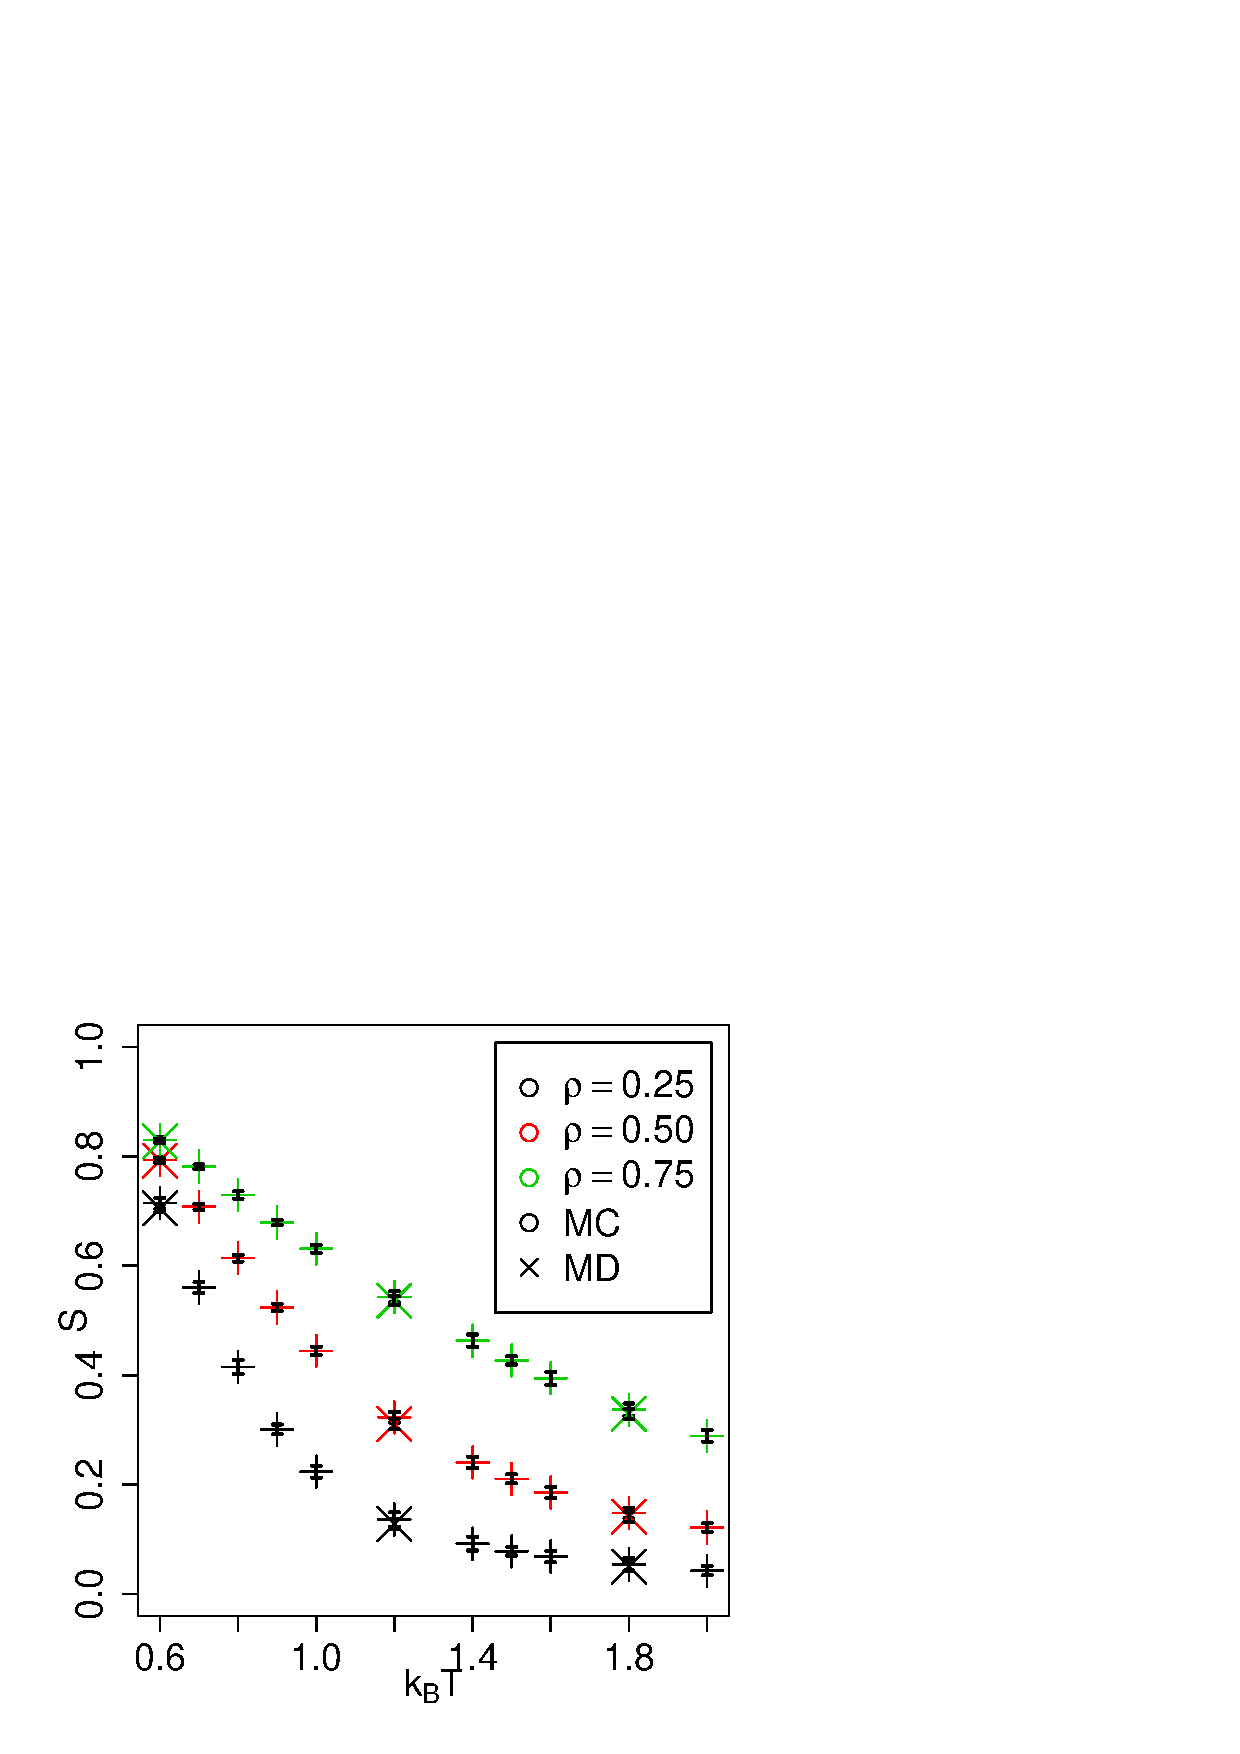
\includegraphics[width=0.8\textwidth]{Images/op_kbt.png}
%	\captionsetup{justification=centering, width=0.9\columnwidth}
%	\caption{Order parameter defined by eq.~\eqref{eq:nematic_order_parameter} versus $k_BT$ for monte-carlo and molecular dynamics simulations. Averaged over 40 samples from which the results were taken on 10 different times}
%	\label{fig:op_kbt}
%\end{figure}

%\begin{figure}[t]
%	\centering
%	\includegraphics[width=0.8\textwidth]{Images/op_from_coaligned.png}
%	\captionsetup{justification=centering, width=0.9\columnwidth}
%	\caption{Order parameter defined by eq.~\eqref{eq:nematic_order_parameter} versus simulation time for different $k_BT$. Points represents molecular dynamics, solid lines shows order parameter obtained from Monte-Carlo}
%	\label{fig:op_from_coaligned}
%\end{figure}

Important to notice that relaxation of the order parameter towards equilibrium if system is started from fully aligned state first taakes leap towards less-aligned state and then gradually increases towards the Monte-Carlo result.

%\begin{figure}[p]
%	\centering
%	\includegraphics[width=0.8\textwidth]{Images/Picture_Data_11.png}
%	\captionsetup{justification=centering, width=0.9\columnwidth}
%	\caption{Langevin Dynamics simultion system evolution for a low temperature $k_BT = 0.5$. The simulation runs from fully-aligned state at the zero time to $2^5$ simulation time units. Time evolution goes from bottom to top}
%	\label{fig:time_evolution_low}
%\end{figure}
%
%\begin{figure}[p]
%	\centering
%	\includegraphics[width=0.8\textwidth]{Images/Picture_Data_16.png}
%	\captionsetup{justification=centering, width=0.9\columnwidth}
%	\caption{Langevin Dynamics simultion system evolution for a high temperature $k_BT = 1.5$. The simulation runs from fully-aligned state at the zero time to $2^5$ simulation time units. Time evolution goes from bottom to top}
%	\label{fig:time_evolution_high}
%\end{figure}